\documentclass[12pt,a4paper]{article}
% This text is inserted in the beginning of all
% LaTex and Tex files I create.
%
% File created: Tue Sep 26 2017
% File name:    report_template.tex
% Path:         /home/name/Classes/AMPIII/Template/
%
% Tayla Broadbridge
% Feb 2022
%

%recommended by fancyhdr package
\setlength{\headheight}{14.49998pt}
\addtolength{\topmargin}{-2.49998pt}

% include a minimal set of useful packages
\usepackage{graphicx}
\usepackage{amsfonts} 
\usepackage{amssymb}
\usepackage{amsmath}
\usepackage[a4paper,margin=3cm]{geometry}
\usepackage{lastpage}
\usepackage{fancyhdr}
\usepackage{listings}
\usepackage{matlab-prettifier}
\usepackage{apacite}
\usepackage{natbib}
%\usepackage[latin1]{inputenc}
\usepackage[english]{babel}
\usepackage[utf8x]{inputenc}
\usepackage{tabularx}
\usepackage{tikz}
\usepackage{graphicx,natbib,amsmath,amsthm,bm,algorithm,algpseudocode,amsfonts,amssymb,bbm,enumitem,blkarray,pgfplots,xcolor,color}
\usepackage{svg}
\usepackage{pdftexcmds}
\usetikzlibrary{automata,positioning}



\begin{document}
\section{Two-island literature review}
The $n$-island model was developed by Sewall Wright \cite{slarkin1985gene} and models the interactions between $n$ populations that have a social structure. An $n$-island structure means that a total population is divided in to $n$ disjoint groups, and these groups of individuals (or genes) can interact with one another through migration. It has been studied by various researchers since its development, including ... \textcolor{red}{who has studied the n-island model? What were they researching specifically?} \cite{arredondo2021inferring} where it has been used to infer demographic history of genes. \\

Since the island model assumes social structure, it is more accurately representative of a true population in comparison to the Wright-Fisher population model which assumes no population structure. Most species display population structure to some extent, which is why the $n$-island model is more useful in such instances. That is, genes reproduce with other individuals that are in physical proximity. In humans, for example, the probability of mating within the same continent is larger than mating between them. On the other hand, for plant species, the probability of pollination is larger for individual plants close together than for individual plants at opposite ends of the field \cite{hein2004gene}. \\

Wright's infinite island model has also been used to study evolutionary game dynamics (cite Ohtsuki, 2010). \\

``The simplest model is that in which the total population is assumed to be divided into subgroups, each breeding at random within itself, except for a certain proportion of migrants drawn at random from the whole \citep{wright1943isolation}.''

\section{My work}
We seek to understand the ancestral genealogy of a population by starting with a current day sample and looking backwards in time. Coalescent theory aims to answer questions about this ancestry and the behaviour of populations. Genealogical quantities of interest are introduced, including tree height and total branch length, and their biological interpretation is discussed. One of the simplest models to describe the genealogical relationship among genes over a series of generations was introduced by \textcolor{red}{Wright (1931) and Fisher (1930)}. This reproductive model describes the evolution of a population and hence the transmission of genes through subsequent genes in discrete time (see HERE for more information about this model). \textcolor{red}{The continuous time coalescent...} From this Wright-Fisher model the continuous time coalescent is derived, where quantities of interest are 
\begin{itemize}
    \item Expected tree height and
    \item Total branch length.
\end{itemize}

Throughout the following section we will consider a coalescent process such that the underlying genealogy follows the two-island model. By looking backwards-in-time we therefore consider coalescent events as well as migration events. We will denote our populations as Island 1 and Island 2. We define the following rate parameters:

\begin{itemize}
    \item $M$, rate at which a single gene migrates from Island 1 to Island 2,
    \item $R$, the rate at which a single gene migrates from Island 2 to Island 1,
    \item $\alpha$, the rate at which a single gene can coalesce on Island 1,
    \item $\beta$, the rate at which a single gene can coalesce on Island 2,
\end{itemize}

and we suppose $i=I_1+I_2$ represents total population size, where $I_1$ and $I_2$ are population sizes of Island 1 and Island 2, respectively. Figure \ref{island_state_diagram} shows the dynamics of such a population.

\begin{figure}[H]
\centering
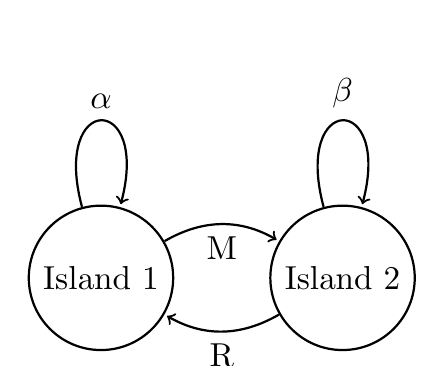
\begin{tikzpicture}[thick,scale=1.2, every node/.style={transform shape}] %Fix scale
        % Draw the states
        \node[state]             (s) {Island 1};
        \node[state, right=of s] (r) {Island 2};
        % Connect the states with arrows
        \draw[every loop]
            (s) edge[loop above] node {$\alpha$} (s)
            (r) edge[loop above] node {$\beta$} (r)
            (s) edge[bend left, auto=right] node {M} (r)
            (r) edge[bend left, auto=left] node {R} (s);
\end{tikzpicture}
\label{island_state_diagram}
\caption{\textcolor{red}{Fix this diagram to make it more intuitive!!!}}
\end{figure}

\textcolor{red}{What are some descriptors of the two-island model?}


The Island Model introduced by *Sewall Wright (1951)* has proven to be a useful construction for studying the interaction of genetic drift, population subdivision, and mutation. 

\subsection{Coalescence and the island model}
Coalescent models have been studied in the context of the island-model/models of segregation. \cite{wakeley2001coalescent} investigated the coalescence in an island model of population subdivision (with variation amongst Demes/groups). \\

Wilkinson-Herbots 1998: The structured coalescent is used to calculate some quantities relating to the genealogy of a pair of homologous genes and to the degree of subpopulation differentiation, under a range of models of subdivided populations and assuming the infinite alleles model of neutral mutation. In this paper they list theoretical values of coalescence times for a range of models of population structure. \\

Wilkinson-Herbots 1998: If $c_1=c_2$ (note $c=c_1+c_2$ where the rate of coalescence between any two genes in sub-population $i$ is $\frac{1}{c_i}$) "c can be considered as the relative population size". In this paper we have listed the theoretical values of coalescence times and FST for a range of models of population structure. They show that in the two-population model, the mean coalescence time of a pair of genes from the larger subpopulation is larger than $c$ (the total population size) (is this measured in generations?), while the mean coalescence time of two genes from the smaller subpopulation is smaller than $c$.

Wakeley 2001: The structured coalescent provides a basis for studying the genealogical history of a sample from a population that is divided into discrete demes (groups) among which there is some pattern of migration. Wilkinson-Herbots (1998) gives an excellent discussion of this model, which is a generalization of Kingman's (1982a, b) ``n-coalescent'' \citep{wakeley2001coalescent}. \\

 Alcala et al. 2019: In this study, we investigate all small network motifs: the set of all possible migration networks among populations subdivided into at most four subpopulations. For each motif, we use coalescent theory to derive expectations for three quantities that describe genetic variation: nucleotide diversity, FST (a measure of population differentiation due to genetic structure), and half-time to equilibrium diversity. \textcolor{red}{So three main quantities that people are interested in when looking at the island model are nucleotide diversity, FST and half-time to equilibrium distribution?}

 \section{Embedding it in a Markov jump process}
The time epochs in betwen coalescent events are exponentially distributed units of time, denoted $T_k \sim \mbox{Exp}(\lambda_k)$. For the case of the Kingman's coalescent, we have that any two genes merge (to find a common ancestor) at rate $T_k \sim \mbox{Exp}(\binom{k}{2})$. This process can hence be represented as a continuous time Markov jump process, where the jump rates are $T_k$, and the jump from state $n-1$ to $n$ represents the jump into our absorption state whereby the $n$ initial genes have found their common ancestor $n$ generations back in time. The underlying CTMC can only transition forward from state $k$ to state $(k+1)$, for all $k = 1,2,\ldots,n-1$, since we are counting the tree height one generation at a time. This is why the time until absorption is the sum of the individual occupation times, $T_k$, for $k=n,n-1,\ldots,2$. The transition matrix for this CTMC is represented as 

\begin{align}
    A = \quad \begin{blockarray}{cccccccc}
    \begin{block}{c(ccccccc)}
    & -\binom{n}{2} & \binom{n}{2} &  & & & &\\ 
    \\
     &  & -\binom{n-1}{2} & \binom{n-1}{2} &  & & &\\
     \\
     & &  & -\binom{n-2}{2} & \binom{n-2}{2} & & &\\
                    & & & &\ddots & \ddots& & \\
                    & & & & & & & \\
                    & & & & & & & \\
                    & & & & & & & -\binom{2}{2} \\ 
           \end{block}
\end{blockarray}.
\label{KingmanMatrix}
\end{align}

We are interested in the time until extinction, $T_n$, representing the time at which we find the MRCA of the $n$ initial genes. See \textcolor{red}{this citation} for the derivation from the discrete-time coalescence. \\

We will now discuss more thoroughly the intensities in (\ref{KingmanMatrix}). Recall that the time between coalescent events are exponentially distributed with a rate which depends on the number of genes in the current population. For the case of the Kingman's coalescent, we have that $T_k \sim \mbox{Exp}\left(\binom{k}{2}\right)$. That is, any $2$ of the $k$ genes in the current population can coalesce. Thus, we have
\begin{enumerate}%[label=\Alph*]
    \item The first exit intensity is 
    \begin{equation*}
        \binom{n}{2}=\frac{n(n-1)}{2},
    \end{equation*}
    representing the rate at which the first event of coalescence occurs whereby the population decreases from $n$ to $n-1$. 
    \item Similarly, the second exit intensity is
    \begin{equation*}
        \binom{n-1}{2}=\frac{(n-1)(n-2)}{2},
    \end{equation*}
    representing the rate at which the second event of coalescence occurs, whereby the population size decreases from $n-1$ to $n-2$. 
    \end{enumerate}
    $\quad \vdots$
    %\setItemnumber{[(a)]}
    \begin{enumerate}
    \item[k.] In general, the $k^{th}$ event of coalescence occurs at rate
    \begin{equation*}
        \binom{n-k+1}{2}=\frac{(n-k+1)(n-k)}{2},
    \end{equation*} which represents the rate at which the population decreases from size $n-k+1$ to $n-k$.
    \end{enumerate}


\subsection{The 2-island model}
We are interested in a 2-island population whereby the initial population is separated into two distinct populations whereby migration can occur. A continuous-time Markov jump process, $\{X_t, t\geq 0\}$, is used to describe the genealogical process in such a model. We suppose that $i=I_1+i_2$ represents the total population size, where $I_1$ and $I_2$ are the number of genes on both $I_1$ and $I_2$ at any given time, respectively. We consider a population whereby genes can migrate and events of coalescence occur on each island according to the dynamics of Kingman's coalescent (cite). The transition rate for any event is 
\begin{equation}
\lambda_{i,I_2} = \binom{i-I_2}{2}\alpha + \binom{I_2}{2}\beta + (i-I_2)M + I_2R.
\end{equation}
Suppose we begin with population size $i=n$. The first event, whether it be an event of migration or coalescence, occurs at rate 
\begin{equation*}
    \lambda_{n,I_2} = \binom{n-I_2}{2}\alpha + \binom{I_2}{2}\beta + (n-I_2)M + I_2R,
\end{equation*}
where 
\begin{itemize}
    \item any two of the $n-I_2$ genes on $I_1$ will coalesce with probability
    \begin{equation*}
        \frac{\binom{n-I_2}{2}}{\lambda_{n,I_2}}
    \end{equation*} such that $n-I_2 \geq 2$,
    \item any two of the $I_2$ genes on $I_2$ will coalesce with probability
    \begin{equation*}
        \frac{\binom{I_2}{2}}{\lambda_{n,I_2}}
    \end{equation*}
    \item one of the genes on Island 1 will migrate to Island 2 with probability 
    \begin{equation*}
        \frac{(n-I_2)M}{\lambda_{n,I_2}}, and
    \end{equation*}
    \item one of the genes on Island 2 will migrate to Island 1 with probability
     \begin{equation*}
        \frac{(I_2R)}{\lambda_{n,I_2}}.
    \end{equation*}   
\end{itemize}

We denote the states of this CTMC as $S=(I_1,I_2)$ and show these possible states in the table:

\begin{table}[h!]
\begin{center}
\begin{tabular}{ |c|c|c| } 
 \hline
 Population size & State  \\
 \hline
$i=n$ & $(n,0)$   \\ 
      & $(n-1,1)$  \\ 
      & $(n-2,2)$  \\ 
      & \vdots \\
      & $(1,n-1)$  \\
      & $(0,n)$  \\
\hline
$i=n-1$ & $(n-1,1)$ \\
 & $(n-2,2)$  \\
 & $(n-3,3)$  \\
 & \vdots   \\
  & $(2,n-2)$ \\
 & $(1,n-1)$ \\
 \hline 
 $i=n-2$ & $(n-2,2)$ \\
 & $(n-3,3)$  \\
 & $(n-4,4)$ \\
 & \vdots  \\
& $(3,n-3)$ \\
& $(2,n-2)$ \\
\hline 
& \vdots  \\
& \vdots  \\
\hline 
$i=2$ & $(2,0)$  \\
& $(1,1)$  \\
& $(0,2)$  \\
\hline
\end{tabular}
\caption{States of the two-island model and their corresponding rewards.}
\label{StatesTable}
\end{center}
\end{table}

Each state within this CTMC is transient with absorbing state(s) when $i=1$

\begin{figure}
    \centering
    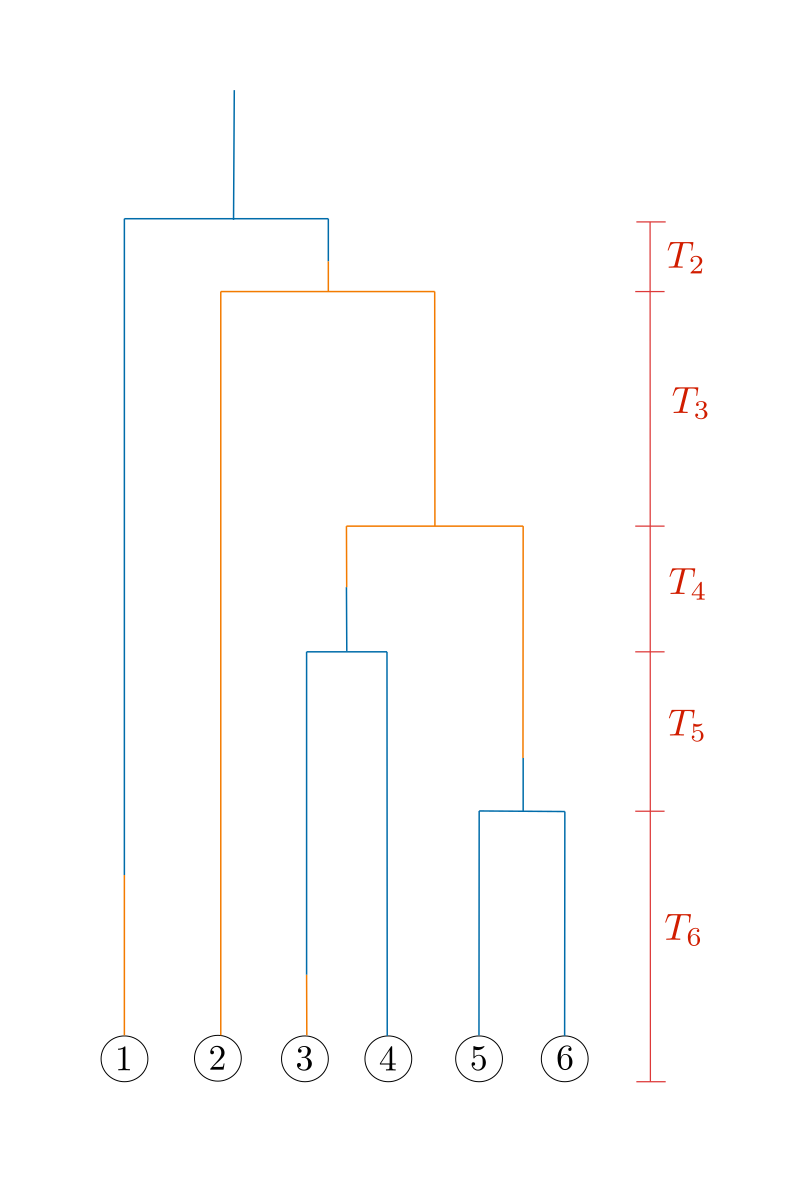
\includegraphics[width=\textwidth]{TwoIslandConstructionColours}
    \caption{A coalescent tree representing a genealogical process described above....... Initially, $i=6$, $I_1=3$ and $I_2=3$.}
   \label{TwoIslandTree}
\end{figure}

Now, to construct our sub-intensity matrix for tree height, we firstly define the $(i+1) \times (i+1)$ matrix
%Gamma is a (i+1) x (i+1) matrix
\begin{center}
\begin{align}
    \Gamma(i) = \quad \begin{blockarray}{cccccccccc}
    %& 0* & 1* & 2* & 3* & \dots & & (T-1)* & T*\\
    \begin{block}{c(ccccccccc)}
     & -\lambda_{i,0} & iM &  & & & & \\ 
     & R & -\lambda_{i,1} & (i-1)M &  & & & \\
     & & 2R & -\lambda_{i,2} & (i-2)M & & &\\
    %3* & &    & 3K & -\lambda_{i,3} & (i-3)c & & & & & \\
                   & & &\ddots & \ddots& \ddots & & & \\
                    & & & & & & & \\
                      & & & &  & & & \\
                       & & & &  & & & \\
                    & & & & & &-\lambda_{i,i-1} & M\\
                    & & & & &  & iR & -\lambda_{i,i} \\ 
           \end{block}
\end{blockarray} 
\end{align}
\end{center}
along with the $(i+1) \times i$ matrix
\begin{align}
    D(i) = \quad \begin{blockarray}{cccccccc}
    %& 0 & 1 & 2 & \cdots & & T \\
    \begin{block}{c(ccccccc)}
      & \alpha\binom{i}{2} & & & & \\
     \\
     & & \alpha\binom{i-1}{2} & & & \\
    \\
     & &\beta\binom{2}{2} & \alpha\binom{i-2}{2} & & & \\
    \\
     & & & \beta\binom{3}{2} & \alpha\binom{i-3}{2} & \\
    & & & &\beta\binom{4}{2} &\ddots & & \\
    & & & & &\ddots & \\
    \\
   & & & & & & 0 \\ 
    \end{block}
    \end{blockarray}
\end{align}
where the parameters $M$, $R$, $\alpha$ and $\beta$ are as defined above. We fit our $\Gamma(i)$ and $D(i)$ matrices together to represent the sub-intensity matrix for tree height in the same way as for the seed-bank coalescent. We thus have that 
\begin{align*}
B(i) = \begin{pmatrix}
\Gamma(i) & D(i) & & & \\
          & \Gamma(i-1) & D(i-1) & & & \\
          &             & \Gamma(i-2) & D(i-2) & & & \\
          & & & \ddots & \ddots & & \\
          & & & & & & \\
          & & & & & & D(3)\\
          & & & & & & \Gamma(2)
\end{pmatrix}
\end{align*}
where
\begin{enumerate}
    \item[(1)] Row $1$ corresponds to the states whereby there are $i=n$ genes in the total population,
    \item[(2)] Row $2$ corresponds to the states whereby there are $i=n-1$ genes in the total population, and \\
    
    \: \vdots
    
    \item[(k)] Row $k$ corresponds to the state whereby there are $i=n-k$ genes in the total population.
\end{enumerate}





\clearpage
\bibliographystyle{apacite}
\bibliography{TwoIsland}




\end{document}